\documentclass[10pt]{article}
\usepackage[latin1]{inputenc}
\usepackage{geometry}                % See geometry.pdf to learn the layout options. There are lots.
\geometry{letterpaper}				% Activate for for rotated page geometry
%\geometry{landscape}
%\usepackage[parfill]{parskip}		% Activate to begin paragraphs with an empty line rather than an indent
\usepackage{graphicx}
\usepackage{epstopdf}
\usepackage{mathptmx}
\usepackage{mathtools}
\usepackage{float}
\usepackage{dblfloatfix}
\usepackage{amsmath}
\usepackage{amsfonts}
\usepackage{amssymb}
\usepackage{multicol}
\usepackage{wrapfig}
\usepackage{amsmath}
\DeclareGraphicsRule{.tif}{png}{.png}{`convert #1 `dirname #1`/`basename #1 .tif`.png}

\begin{document}
\title{Upper Atmosphere and Ionosphere Assignment 5}
\author{Jillian S. Estrella}
\date{April 27, 2012}
\maketitle

\section{Introduction}
In order to improve upon the existing ionosphere structure developed in HW4, I attempted to add electron and ion cooling rates. I calculate these terms to develop a more accurate equation for energy dissipation in the previously derived tridiagonal matrix for electron temperature. I also add a tridiagonal matrix for ion temperature and similarly add/subtract terms to/from the ion energy dissipation.

\section{Background}
\subsection{Tridiagonal Matrix for Ion Temperature}
I essentially used the same tridiagonal matrix for the ions as I did for the electrons. The only major difference is that I used the following thermal conductivity for ions provided in class

\begin{equation}
\lambda _{i} = \frac{4.6 \times 10^{4} T_{i}^{5/2}}{A_{i}^{1/2}}
\end{equation}

\noindent Where A$_{i}$ is the atomic weight given in units of [AMU].

\subsection{Developing the Appropriate Momentum Transfer Collision Frequencies}
I began by identifying the equations for calculating the appropriate loss terms. Using equation 4.129c in Schunk \& Nagy, one of the linear collision terms for the 13 moment approximation.

\begin{equation}
\frac{\delta E_{s}}{ \delta t} = - \Sigma \frac{n_{s}m_{s}\upsilon _{st}}{m_{s} + m_{t}} 3k(T_{s}-T_{t})
\end{equation}

\subsection{Calculating Collision Frequencies}
Equation 4.129c in Schunk \& Nagy is dependent upon collision frequency. I identified the appropriate collision frequency based on the nature of the interaction (ie. electron-ion, electron-neutral, etc.). I considered the necessary interactions and evaluate the given equations for each species taken from Shunk \& Nagy.

\noindent For the electron(cool)-neutral(heat) interaction we have

\begin{equation}
\upsilon _{eN_{2}} = 2.33\times 10^{-11}n(N_{2})(1-1.21\times 10^{-4}T_{e})T_{e}
\end{equation}


\begin{equation}
\upsilon _{eO_{2}} = 1.82\times 10^{-10}n(O_{2})(1+3.6\times 10^{-2}T_{e}^{1/2})T_{e}^{1/2}
\end{equation}


\begin{equation}
\upsilon _{eO} = 1.82\times 10^{-10}n(O)(1+3.57\times 10_{-4}T_{e})T_{e}^{1/2}
\end{equation}

\noindent For the neutral(cool)-ion(heat) interactions we have


\begin{equation}
\upsilon _{O^{+}O} = 3.67\times 10^{-11}n(O)T_{r}^{1/2}(1-0.064log_{10}T_{r})^{2}T_{e}^{1/2}
\end{equation}


\begin{equation}
\upsilon _{N_{2}^{+}N_{2}} = 5.14\times 10^{-11}n(N_{2})T_{r}^{1/2}(1-0.069log_{10}T_{r})^{2}T_{e}^{1/2}
\end{equation}


\begin{equation}
\upsilon _{O_{2}^{+}O_{2}} = 2.59 \times 10^{-11}n(O_{2})T_{r}^{1/2}(1-0.073log_{10}T_{r})^{2}T_{e}^{1/2}
\end{equation}


\noindent In these equations the average temperature, $T_{r}$, is

\begin{equation}
T_{r}= \frac{T_{i} + T_{n}}{2}
\end{equation}

\noindent For the electron-ion interaction the following equation applies

\begin{equation}
\upsilon _{ei}= 54.5\frac{n_{i}Z_{i}^{2}}{T_{e}^{3/2}}
\end{equation}

\noindent Z, particle charge number, is equal to one in this instance because all ions are singly charged.
\\

\noindent When calculating the ion-neutral interactions we must consider both resonant and non-resonant collision frequencies.  They are taken from Schunk \& Nagy Table 4.5 and equation 4.146 respectively.

\begin{equation}
\upsilon _{in}= C_{in}n_{n}
\end{equation}

\noindent The coefficients are taken from Schunk \& Nagy Table 4.4.

\subsection{Electron Cooling Rates}
Chapter 9 in Schunk \& Nagy provides electron cooling rates. I calculated these values for the N$_{2}$ rotation, O$_{2}$ rotation, O$_{2}$ vibration, and O fine structure contributions. It should be noted that I attempted to calculate the N$_{2}$ vibration contribution with no success. The above mentioned equations are
\\

\noindent N$_{2}$ rotation

\begin{equation}
L_{e}(N_{2})=\frac{3.5 \times 10^{-14}n_{e}n(N_{2})(T_{e}-T_{n})}{T_{e}^{1/2}}
\end{equation}

\noindent O$_{2}$ rotation

\begin {equation}
L_{e}(O_{2})=\frac{5.2 \times 10^{-15}n_{e}n(O_{2})(T_{e}-T_{n})}{T_{e}^{1/2}}
\end {equation}

\noindent O$_{2}$ vibration

\begin{equation}
L_{e}(O_{2})=n_{e}n(O_{2})Q(T_{e})\{1-exp{[2239(T_{e}^{-1}-T_{n}^{-1})]}
\end{equation}

\noindent Where

\begin{equation}
\begin{split}
\log _{10} [Q(T_{e})] =& \left( -19.9171 + 0.0267T_{e} - 3.9960 \times 10^{-5}T_{e}^{2} \right. \\ & \left.
+ 3.5187 \times 10^{-8}T_{e}^{3} - 1.9228 \times 10^{-11}T_{e}^{4} \right. \\ & \left.
+ 6.6865 \times 10^{-15}T_{e}^{5} - 1.4791 \times 10^{-18}T_{e}^{6} \right. \\ & \left.
+ 2.0127 \times 10^{-22}T_{e}^{7} - 1.5346 \times 10^{-26}T_{e}^{8} \right. \\ & \left.
+ 5.0148 \times 10^{-31}T_{e}^{9} \right)
\end{split}
\end{equation}


\noindent Oxygen fine structure

\begin{equation}
\begin{split}
L_{e}(O) =& n_{e} n(O) D^{-1} \left( S_{10} \lbrace 1 - exp{[98.9(T_{e}^{-1} - T_{n}^{-1})]} \rbrace \right. \\ & \left.
+ S_{20} \lbrace 1 - exp[326.6(T_{e}^{-1} - T_{n}^{-1})] \rbrace \right. \\ & \left.
+ S_{21} \lbrace 1-exp[227.7(T_{e}^{-1} - T_{n}^{-1})] \rbrace \right)
\end{split}
\end{equation}

\noindent Where

\begin{equation}
D = 5 + exp{-326.6 T_{n}^{-1}}
\end{equation}

\begin{equation}
S_{21} = 1.863 \times 10^{-11}
\end{equation}

\begin{equation}
S_{21} = 1.191 \times 10^{-11}
\end{equation}

\begin{equation}
S_{21} = 8.249 \times 10^{-11}
\end{equation}

\subsection{Energy Dissipation}
Upon calculating all quantities we add or subtract these terms from the already developed equations for energy dissipation, Q, in the tridiagonal matrix. Subtraction or addition of a given term is determined by the source of the exchange (ie. loss or gain).

\section{Results}
The following plots are provided with captions discussing the results.
\begin{figure}[H]
	\centering
		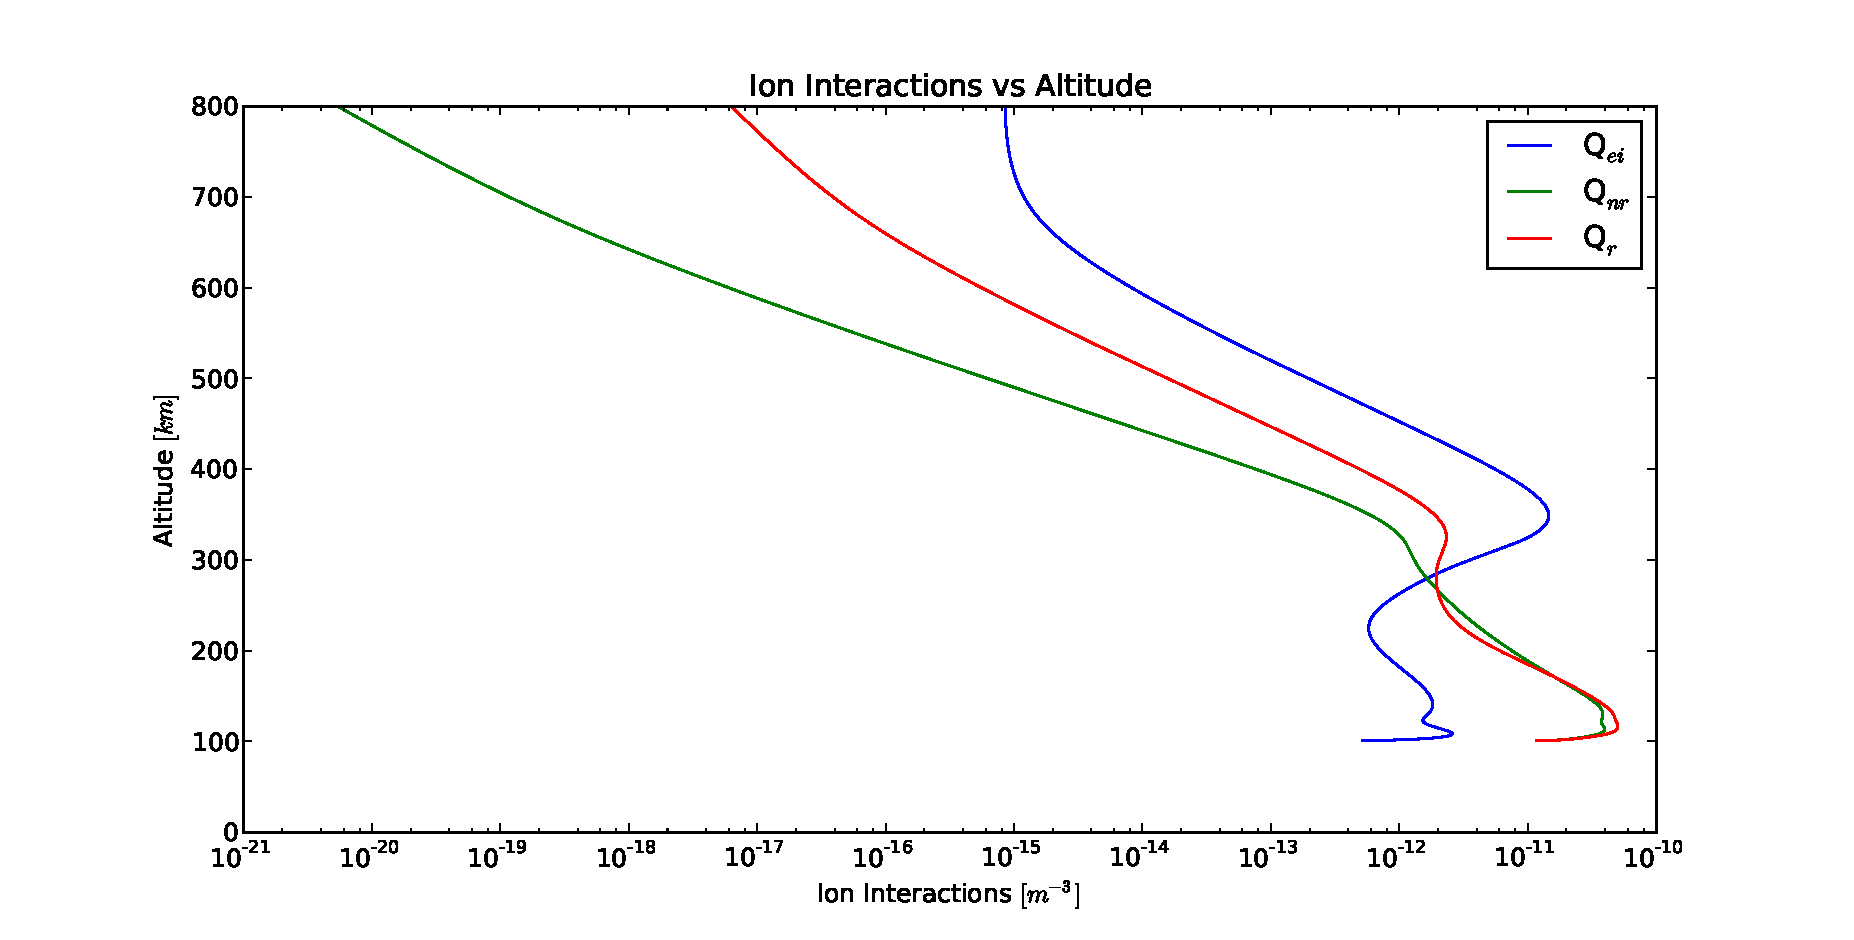
\includegraphics[width=0.99\textwidth]{../Figures/B/Ion_Interactions_vs_Altitude.eps}
	\caption{This is a plot of the Ion interactions vs Altitude. I don't have much to say about this because I have no physical intuition regarding what the behavior of these loss terms should look like.}
	\label{fig:n1}
\end{figure}
\begin{figure}[H]
	\centering
		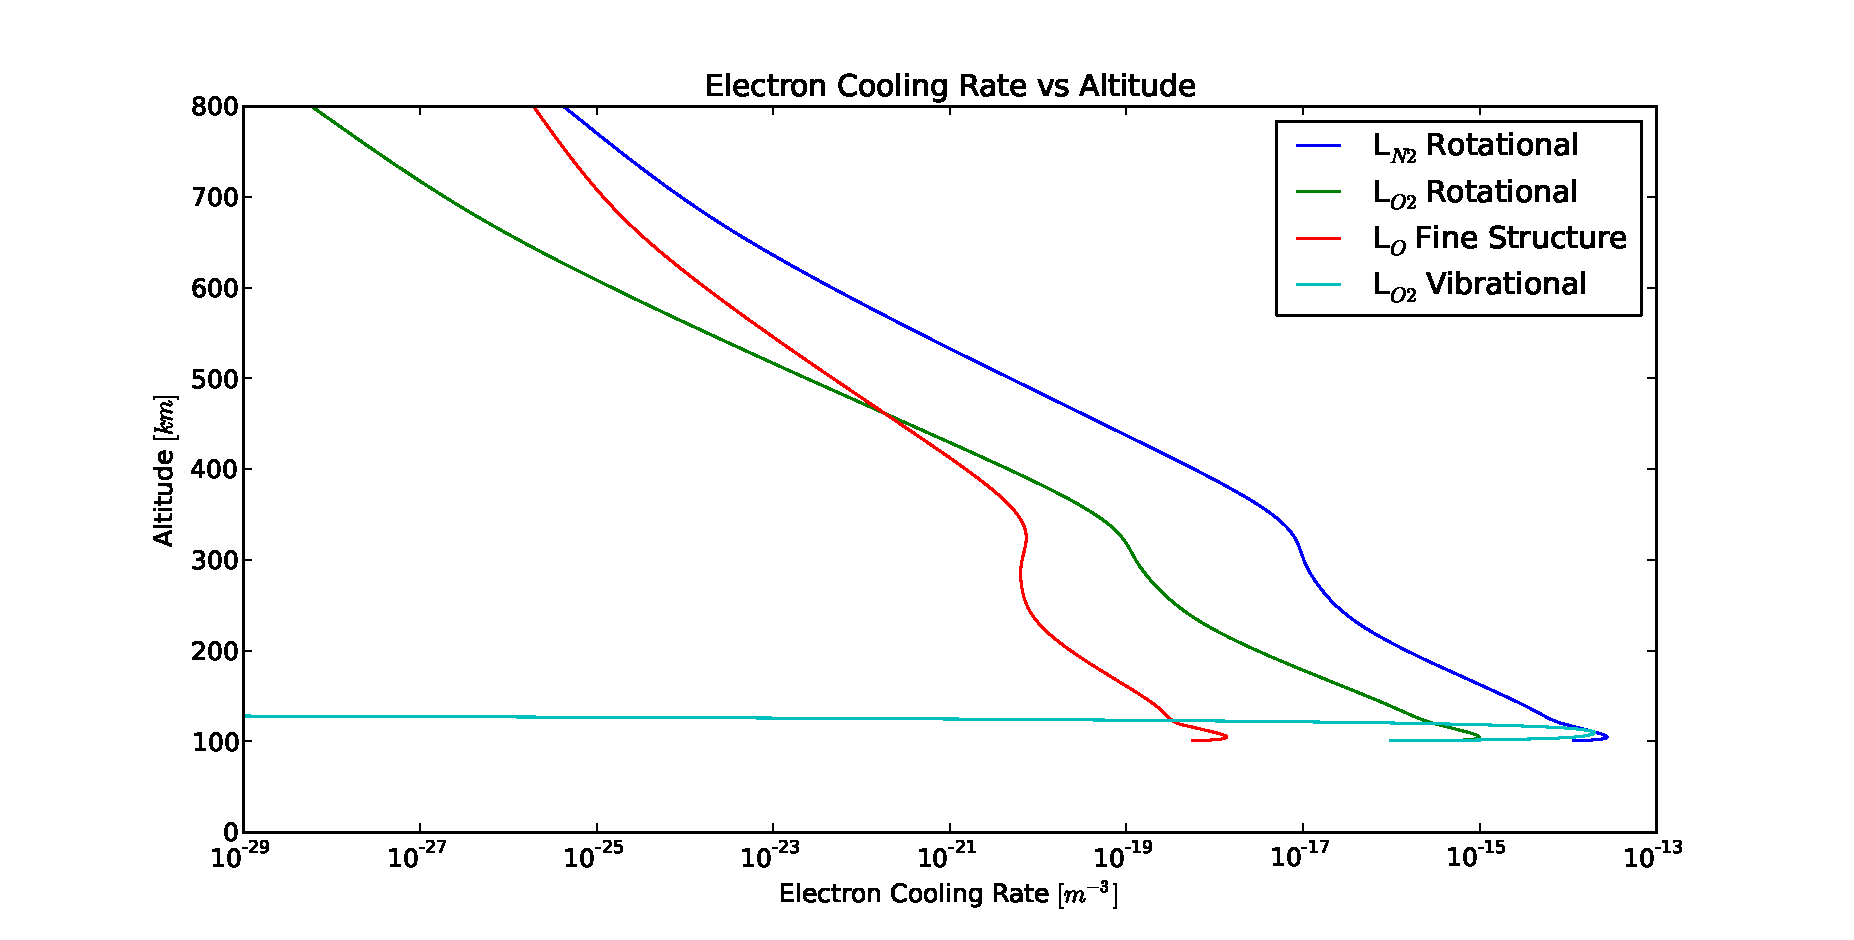
\includegraphics[width=0.99\textwidth]{../Figures/B/Electron_Cooling_Rates_vs_Altitude.eps}
	\caption{These are the electron coolins rates. Again I don't have much to say about this because I have no physical intuition regarding what the behavior of these loss terms should look like. I find it interesting the the L$_{O2}$ term is so small compared to the rest. But this could just mean that the term isn't very important with respect to cooling.}
	\label{fig:n2}
\end{figure}
\begin{figure}[H]
	\centering
		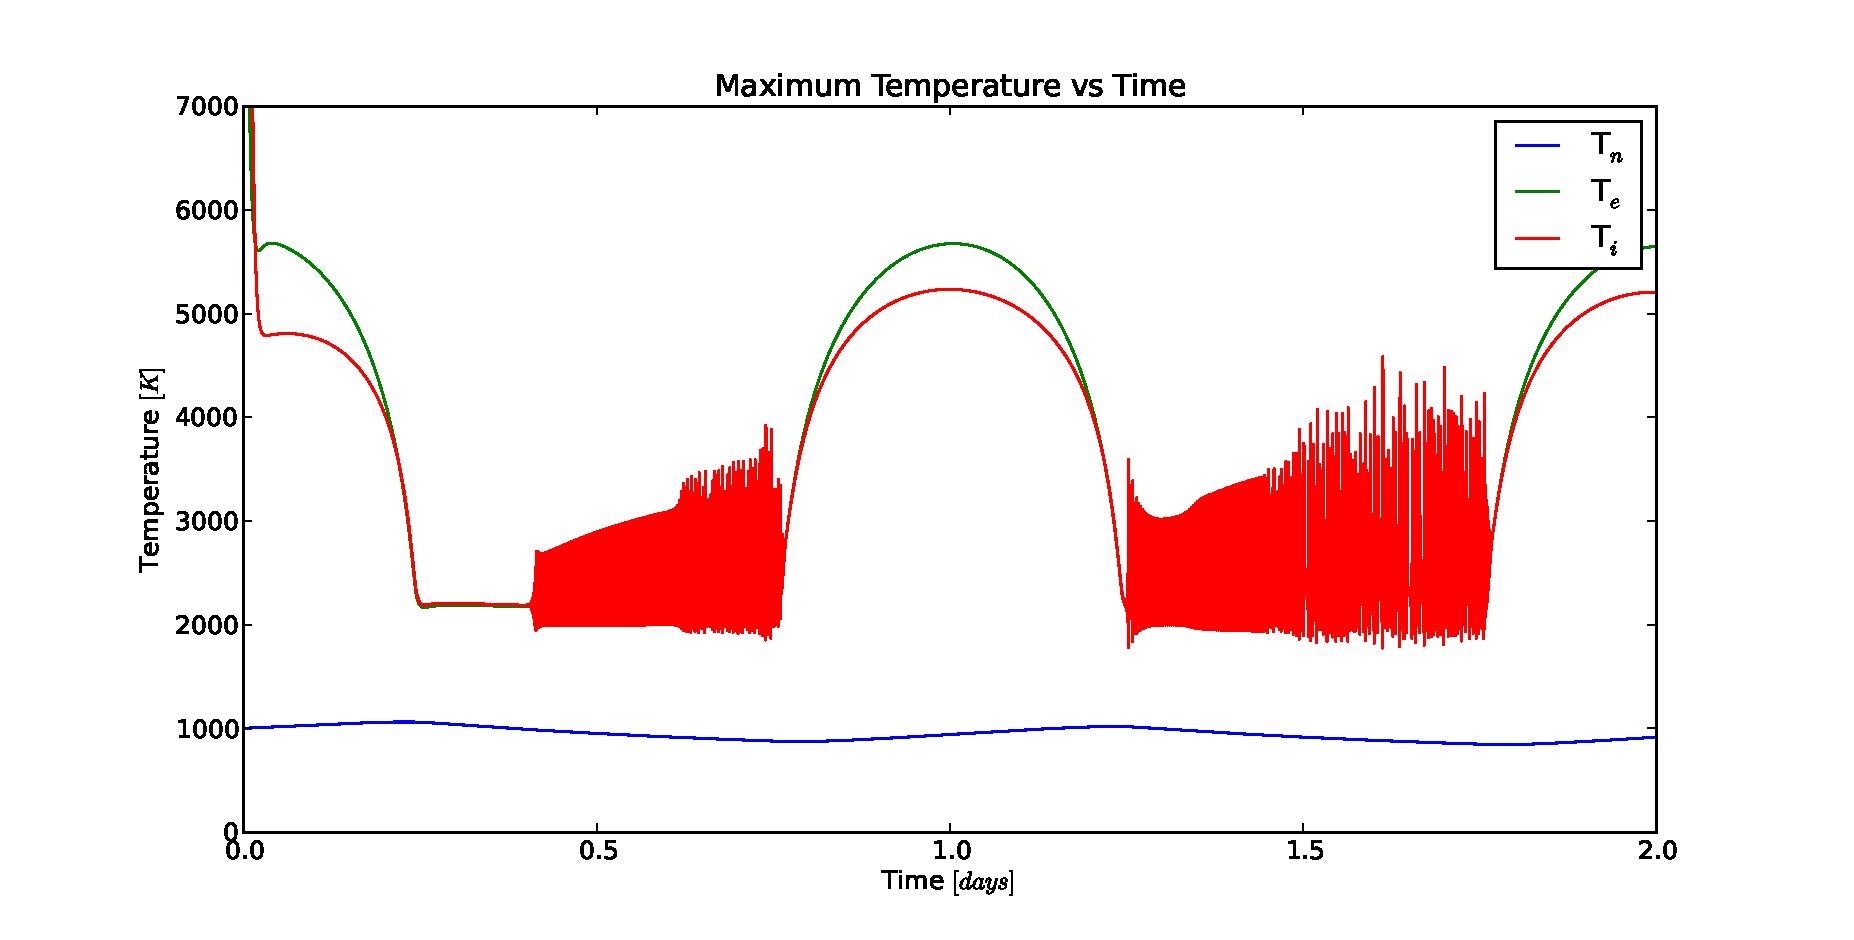
\includegraphics[width=0.99\textwidth]{../Figures/B/T_max_vs_time.eps}
	\caption{This is a plot of Maximum Temperature vs Time. I believe that this plot is the most important regarding my results. As you can see I ran my model over a period of two days in an attempt to flush out any numerical quirks. For some reason the ion temperature is not behaving very well. This is clearly due to a numerics problem.}
	\label{fig:n3}
\end{figure}

\section{Discussion \& Conclusion}
This was a difficult assignment. I must admit that I did not get things working how they should. In order to get the ion temperature to do something somewhat well behaved I had to fudge a few orders of magnitude in the ion interaction terms. Even with this fudge factor they still do not behave how they should. As previously mentioned I also couldn't get the N$_{2}$ vibration contribution to work. My intuition tells me that the elevtron temperatures are close to what they should be. By adding the N$_{2}$ vibration contribution I cannot predict how much this will alter the results. On the other hand the ion temperatures shown above are far too hot. If I were able to find what was going wrong with my ion temperature calculation I believe that they would be much cooler than the electrons (yet still hotter than the neutrals).

\end{document}
